In this section we will describe the datasets used and the pipeline, including pre-processing and feature extraction, 

\subsection{Datasets}
In our experiments we use three datasets, each assigned to a model as described in Table\ref{tbl:datasets}. The datasets used are public and provide audio clips of different lengths and quality.

\begin{table}[!h]
\centering
\caption{Description of datasets used in our experiments. Book narr. refers to book narratives. Newspaper ++ refers to newspapers and other documents. Conversational tel. refers to conversational telephone speech.}
\label{tbl:datasets}
\begin{tabular}{llllll}
                                                                     & \cellcolor[HTML]{C0C0C0}Speakers & \cellcolor[HTML]{C0C0C0}Language & \cellcolor[HTML]{C0C0C0}Duration & \cellcolor[HTML]{C0C0C0}Context & \cellcolor[HTML]{C0C0C0}Model \\ \cline{2-6} 
\multicolumn{1}{l|}{\cellcolor[HTML]{C0C0C0}2013 Blizzard} & 1                                & English                          & 73 h                             & Book narr.                  & SampleRNN                     \\
\multicolumn{1}{l|}{\cellcolor[HTML]{C0C0C0}CSTR VCTK}               & 109                              & English                          & 400 Sentences                    & Newspaper ++               & WaveNet                       \\
\multicolumn{1}{l|}{\cellcolor[HTML]{C0C0C0}2004 NIST}               & 100                              & Multiple                         & 5 min / speaker                  & Conversational tel. & WGAN                         
\end{tabular}
\end{table}

\subsection{Pre-processing}
\label{sub:processdata}
Data pre-processing is dependent on the model being trained. For SampleRNN and WaveNet, the raw audio is reduced to 16kHz and quantized using the $\mu-law$ companding transformation as referenced in SampleRNN~\cite{mehri2016samplernn} and WaveNet~\cite{van2016wavenet}. For the model based on the Wasserstein GAN, we pre-process the data by converting it to 16kHz and removing silences by using the WebRTC Voice Activity Detector (VAD) as referenced in~\cite{zeidan2014webrtc}.

\subsection{Feature extraction}
SampleRNN and WaveNet operate at the sample level, i.e. waveform, thus requiring no feature extraction.
The features used for the neural speaker recognition system is based on Mel-Spectrograms with dynamic range compression. The Mel-Spectrogram is obtained by projecting a spectrogram onto a mel scale. We use the python library librosa~\cite{mcfee2015librosa} to project the spectrogram onto 64 mel bands, with window size equal to 1024 samples and hop size equal to 160 samples, i.e. frames of 100ms long. Dynamic range compression is computed as described in~\cite{lukic2016speaker}, with $log(1 + C*M)$, where $C$ is the a compression constant scalar set to $1000$ and $M$ is the matrix representing the Mel-Spectrogram.
                        
\section{Classification Model}
\subsection{Gaussian Mixture Model - Universal Background Model}
\subsection{Neural speaker recognition system}
The speaker recognition system used in our experiments is based on the state-of-the-art framework by \cite{lukic2016speaker} and is described in Figure \ref{fig:CNN}. The first module at the bottom is a pre-processing step that extracts Mel-Spectrograms features from the waveform as described in section \ref{sub:processdata}. The second module is a convolutional neural network (CNN) that performs multi-speaker classification using the Mel-Spectrograms. The CNN is a modified version of Alexnet~\cite{krizhevsky2012imagenet}.

\begin{figure}[h]
    \centering
    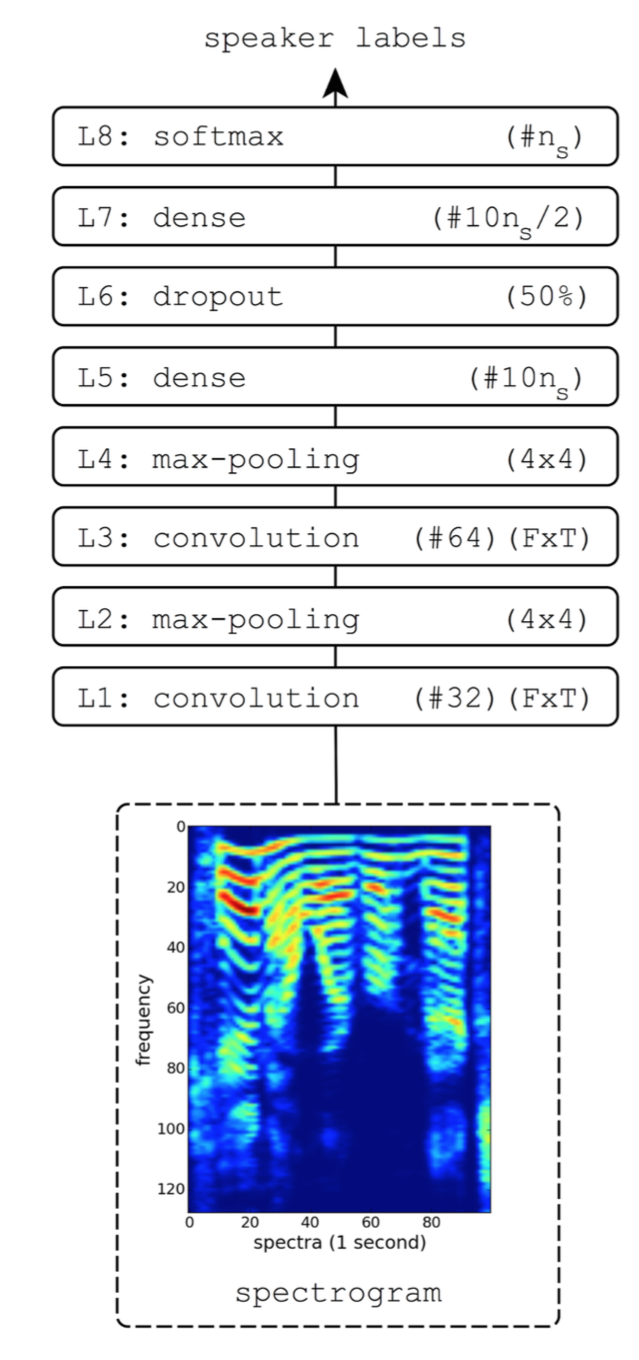
\includegraphics[width=0.25\textwidth]{./fig/cnn.png}
    \caption{Architecture for CNN speaker verifier}
    \label{fig:CNN}
\end{figure}

We train the CNN on our training set using 64*64 Mel-Spectrograms~\footnote{64 mel bands and 64 frames, 100 ms each} consisting of balanced samples from 101 speakers from the NIST 2004 and Blizzard datasets. Our model achieves 85\% test set accuracy.

\section{Generative Model}
\subsection{WaveNet} % (fold)
\label{sub:WaveNet}
WaveNet is a generative neural network trained end-to-end to model quantized audio waveforms. It has produced impressive results for conditional, speaker and text, generation of speech audio. The model is fully probabilistic and autoregressive, using a stack of causal convolutional layers to condition the predictive distribution for each audio sample on all previous ones;
\subsection{SampleRNN}
SampleRNN \cite{mehri2016samplernn}, another autoregressive architecture that has been successfully used to generate both speech and music samples. SampleRNN uses a hierarchical structure of deep RNNs to model dependencies in the sample sequence. Each deep RNN operates at a different temporal resolution so as to model both long term and short term dependencies.  
\subsection{Wasserstein GANs} % (fold)
\label{sub:Wasserstein_GANsh}
In the original generative adversarial network (GAN) framework proposed by \cite{goodfellow2014generative}, a \textit{generator} network is trained to learn a function from noise to samples that approximate the real data distribution. Simultaneously, a \textit{discriminator} network is trained to identify whether a sample came from the real distribution or not - i.e., it is trained to try to output 1 if a sample is real, and 0 if a sample is fake. The generator and discriminator can be arbitrary networks. \\
The GAN framework has been shown to be able to produce very realistic samples with low training overhead. However, since the generator is trained to minimize the Kullback-Leibler (KL) divergence between its constructed distribution and the real one, it suffers from an exploding loss term when the real distribution's support isn't contained in the constructed one. To counter this, the \textit{Wasserstein GAN} \cite{arjovsky2017wasserstein} (WGAN) framework instead uses the Wasserstein (Earth-Mover) distance between distributions instead, which in many cases does not suffer from the same explosion of loss and gradient. Based on this, the loss functions of the generator and \textit{critic} (which no longer emits a simple probability, but rather an approximation of the Wasserstein distance between the fake distribution and real) become:
\begin{align}
    L_G &= -\underset{\boldsymbol{\widetilde{x}} \sim \mathbb{P}_{g}}{\mathbb{E}}  \big[D(\boldsymbol{\widetilde{x}})\big] \\
    L_C &= \underset{\boldsymbol{\widetilde{x}} \sim \mathbb{P}_{g}}{\mathbb{E}}  \big[D(\boldsymbol{\widetilde{x}})\big] - \underset{\boldsymbol{x} \sim \mathbb{P}_{r}}{\mathbb{E}}  \big[D(\boldsymbol{x})\big]
\end{align}
where $P_r$ is the real distribution, and $P_g$ the learnt distribution of the generator. \\
The original WGAN framework uses weight clipping to ensure that the critic satisfies a Lipschitz condition. As pointed by \cite{gulrajani2017improved}, however, this clipping can lead to problems with gradient stability. Instead, \cite{gulrajani2017improved} suggest adding a gradient penalty to the critic's loss function, which indirectly tries to constrain the original critic's gradient to have norm close to 1. Equation (2) thus becomes (taken from \cite{gulrajani2017improved}):
\begin{align}
    L_C &= \underbrace{\underset{\boldsymbol{\widetilde{x}} \sim \mathbb{P}_{g}}{\mathbb{E}}  \big[D(\boldsymbol{\widetilde{x}})\big] - \underset{\boldsymbol{x} \sim \mathbb{P}_{r}}{\mathbb{E}}  \big[D(\boldsymbol{x})\big]}_\text{Original critic loss}  + \underbrace{\lambda \underset{\boldsymbol{\hat{x}} \sim \mathbb{P}_{\hat{x}}}{\mathbb{E}}  \big[(\lVert \nabla_{\boldsymbol{\hat{x}}} D(\boldsymbol{\hat{x}}) \rVert_2 - 1)^2\big]}_\text{Gradient Penalty}
\end{align}

% subsection wgan_approach (end)
\subsection{Adversarial attacks}
Attacks to classification systems can be targeted or untargeted. In targeted attacks, an adversary is interested in producing an adversarial input that makes the classification system predict a target class. In untargeted attacks, the adversary is interest in a confident prediction, regardless of the class.
